% !TEX TS-program = pdflatex
% !TEX encoding = UTF-8 Unicode

% This file is a template using the "beamer" package to create slides for a talk or presentation
% - Giving a talk on some subject.
% - The talk is between 15min and 45min long.
% - Style is ornate.

% MODIFIED by Jonathan Kew, 2008-07-06
% The header comments and encoding in this file were modified for inclusion with TeXworks.
% The content is otherwise unchanged from the original distributed with the beamer package.

\documentclass[handout]{beamer}
\usepackage{pgfpages}
%\pgfpagesuselayout{4 on 1}[a4paper,border shrink=5mm]

% Copyright 2004 by Till Tantau <tantau@users.sourceforge.net>.
%
% In principle, this file can be redistributed and/or modified under
% the terms of the GNU Public License, version 2.
%
% However, this file is supposed to be a template to be modified
% for your own needs. For this reason, if you use this file as a
% template and not specifically distribute it as part of a another
% package/program, I grant the extra permission to freely copy and
% modify this file as you see fit and even to delete this copyright
% notice. 


\mode<presentation>
{
  \usetheme{Warsaw}
  % or ...

  \setbeamercovered{transparent}
  % or whatever (possibly just delete it)
}


\usepackage[english]{babel}
% or whatever

\usepackage[utf8]{inputenc}
% or whatever

\usepackage{times}
\usepackage[T1]{fontenc}
% Or whatever. Note that the encoding and the font should match. If T1
% does not look nice, try deleting the line with the fontenc.

%%% MATH RELATED
\usepackage{amsmath,amsthm,amssymb}
\usepackage{mathrsfs}  
\usepackage[all]{xy}
\newcommand{\bbc}{\mathbb{C}}
\newcommand{\bbr}{\mathbb{R}}
\newcommand{\bbn}{\mathbb{N}}
\newcommand{\M}{\mathscr{M}}
\renewcommand{\L}{\mathcal{L}}
\newcommand{\vocab}[1]{\textbf{#1}}
\newcommand{\Bis}{\text{Bis}}
\newcommand{\spec}{\text{spec}}
\newcommand{\ol}[1]{\overline{#1}}
\newcommand{\wt}[1]{\widetilde{#1}}
\newcommand{\Ad}{\textnormal{Ad}}

\theoremstyle{definition}
\newtheorem{defn}{Definition}
\newtheorem{quest}{Question}
\newtheorem{prob}{Problem}
\newtheorem{obs}{Observation}
\newtheorem{ex}{Example}
\newtheorem{notation}{Notation}
\newtheorem{thm}{Theorem}
\newtheorem{prop}{Proposition}
\newtheorem{cor}{Corollary}

\title{Math Competition Questions 3}

\subtitle
{Math 180 Strategies of Problem Solving}

\author[W.R. Casper] % (optional, use only with lots of authors)
{}%{W.R. Casper}
% - Use the \inst{?} command only if the authors have different
%   affiliation.

\institute[California State University Fullerton] % (optional, but mostly needed)
{
  Department of Mathematics\\
  California State University Fullerton}
% - Use the \inst command only if there are several affiliations.
% - Keep it simple, no one is interested in your street address.

\subject{Talks}
% This is only inserted into the PDF information catalog. Can be left
% out. 



% If you have a file called "university-logo-filename.xxx", where xxx
% is a graphic format that can be processed by latex or pdflatex,
% resp., then you can add a logo as follows:

% \pgfdeclareimage[height=0.5cm]{university-logo}{university-logo-filename}
% \logo{\pgfuseimage{university-logo}}



% Delete this, if you do not want the table of contents to pop up at
% the beginning of each subsection:
\AtBeginSubsection[]
{
  \begin{frame}<beamer>{Outline}
    \tableofcontents[currentsection,currentsubsection]
  \end{frame}
}


% If you wish to uncover everything in a step-wise fashion, uncomment
% the following command: 

%\beamerdefaultoverlayspecification{<+->}


\begin{document}

\begin{frame}
  \titlepage
\end{frame}

%\begin{frame}{Outline}
%  \tableofcontents
%  % You might wish to add the option [pausesections]
%\end{frame}


% Since this a solution template for a generic talk, very little can
% be said about how it should be structured. However, the talk length
% of between 15min and 45min and the theme suggest that you stick to
% the following rules:  

% - Exactly two or three sections (other than the summary).
% - At *most* three subsections per section.
% - Talk about 30s to 2min per frame. So there should be between about
%   15 and 30 frames, all told.

\section{Problem List}
\begin{frame}{Question 1}
\begin{quest}
How many square yards of carpet are required to cover a rectangular floor that this $12$ feet long and $9$ feet wide?  (There are $3$ feet in a yard.)
\end{quest}
\end{frame}

\begin{frame}{Question 2}
\begin{quest}
Jack and Jill are going swimming at a pool that is one mile from their house.  They leave home simultaneously.  Jill rides her bicycle to the pool at a constant speed of $10$ miles per hour.  Jack walks to the pool at a constant speed of $4$ miles per hour.  How many minutes before Jack does Jill arrive?
\end{quest}
\end{frame}

\begin{frame}{Question 3}
\begin{quest}
Billy's basketball team scored the following points of the course of the first $11$ games of the season:
$$42,47,53,53,58,58,58,61,64,65,73.$$
If his team scored $40$ in the $12$'th game, which of the following statistics will show an increase?
$$\text{range},\ \ \text{median},\ \ \text{mean},\ \ \text{mode},\ \ \text{mid-range}$$
\end{quest}
\end{frame}

\begin{frame}{Question 4}
\begin{quest}
Each of two boxes contains three chips numbered $1,2,3$.  A chip is drawn randomly from each box and the numbers on the two chips are multiplied.  What is the probability that the product is even?
\end{quest}
\end{frame}

\begin{frame}{Question 5}
\begin{quest}
On her first day of work, Janabel sold one widget.  On day two, she sold three widgets.  On day three, she sold five widgets, and on the succeeding day, she sold two more widgets than she sold on the previous day.  How many widgets in total had Janabel sold after $20$ days?
\end{quest}
\end{frame}

\begin{frame}{Question 6}
\begin{quest}
In the small country o fIcosahedrontopia, all automobile license plates have four symbos.  The first must be a vowel (A,E,I,O, or U), the second and third must be two different letters aong the 21 non-vowels, and the fourth must be a digit (0 through 9).  If the symbols are chosen at random subject to these conditions, what is the probability that the plate will read ``AMC8"?
\end{quest}
\end{frame}

\begin{frame}{Question 7}
\begin{quest}
How manysubsets of two elements can be removed from the set $\{1,2,3,4,5,6,7,8,9,10,11\}$ so that the mean (average) fo the remaining numbers is $6$?
\end{quest}
\end{frame}

\begin{frame}{Question 8}
\begin{quest}
At Euler Middle School, $198$ students voted on two issues in a school referendum with the following results: $149$ voted in favor fo the first issue and $119$ voted in favor of the second issue.  If there were exactly $29$ students who voted against both issues, how many students voted in favor of both issues?
\end{quest}
\end{frame}

\begin{frame}{Question 9}
\begin{quest}
Jeremy's father drives him to school in rush hour traffic in $20$ minutes.  One day there is no traffic, so his father can drive him $18$ miles per hour faster and gets him to school in $12$ minutes.  How far in miles is it to school?
\end{quest}
\end{frame}

\begin{frame}{Question 10}
\begin{quest}
A triangle with vertices $A=(1,3)$, $B=(5,1)$ and $C=(4,4)$ is plotted in a $6\times 5$ grid.  What fraction of the grid is covered by the triangle?
\end{quest}
\begin{center}
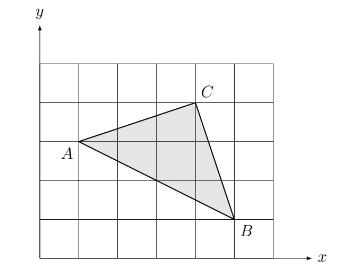
\includegraphics[width=.5\linewidth]{fig/probset3fig1.png}
\end{center}
\end{frame}

\end{document}


